\chapter{Diagramma di macchina a stati}
Le macchine a stati possono essere utilizzate per modellare il comportamento dinamico di classificatori
quali classi, casi d'uso, sottosistemi e interi sistemi.
\\ Le macchine a stati esistono nel contesto di un particolare classificatore che:
\begin{itemize}
    \item Risponde a eventi esterni
    \item Ha un ciclo di vita definito, che può essere modellato come una successione di stati,
    transizioni ed eventi
    \item Può avere un comportamento corrente che dipende dai comportamenti precedenti
\end{itemize}
Le macchine a stati di solito vengono utilizzate per modellare il comportamento
dinamico degli oggetti.
\section{Tipi di oggetti}
\begin{itemize}
    \item Indipendenti dallo stato - Oggeti che rispondono sempre nello statto modo a un determinato evento
    \item Dipendenti dallo stato - Rispondono in modi diversi ad un determinato evento a seconda dello stato
    in cui si trovano
\end{itemize}
\subsection*{Modellazione oggetti dipendenti dallo stato}
Modellano il comportamento di un oggetto reattivo complesso in risposta agli eventi oppure modellano
le sequenze valide delle operazioni ovvero specifiche di protocollo o linguaggio.
\\ Esempi di oggetti complessi sono dispositivi fisici come un telefono o un'auto, oppure
transazioni e oggetti di business (ordine, vendita, pagamenti, ecc.).
\paragraph*{Altri esempi}
\begin{itemize}
    \item Protocolli di comunicazione - TCP si comporta in maniera diversa a seconda dello stato in cui 
    la comunicazione si trova
    \item Flusso e navigazione delle pagine/finestre UI
    \item Controlle di flusso UI
    \item Operazioni di sistema dei casi d'uso - endSale deve arrivare solo dopo una o più operazioni enterItem
\end{itemize}
\section{Macchina a stati - Sintassi e rappresentazione}
Noterete dalla seguente immagine che si tratta praticamente di un DFA 
(Deterministic Finite Automa - Automa a stati finiti deterministico) dove abbiamo:
\begin{itemize}
    \item Uno stato iniziale
    \item Stati intermedi
    \item Transizioni (etichettate da eventi)
    \item Stato finale
\end{itemize}
\begin{center}
    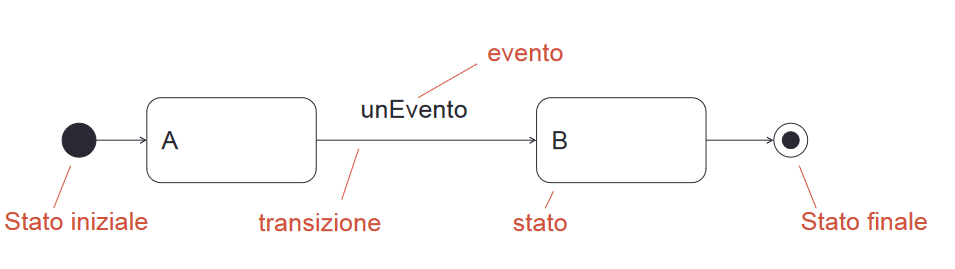
\includegraphics[scale=0.5, width=100mm]{img/macchina_a_stati_syntax.png}
\end{center}
\subsection*{Stati}
Una condizione o una situazione della vita di un oggetto durante la quale tale oggetto soddisfa
una condizione, esegue un'attività o aspetta un evento.
Lo stato di un oggetto in qualsiasi momento è determinato da
\begin{itemize}
    \item I valori dei suoi attributi
    \item Le relazioni che ha con altri oggetti
    \item Le attività che sta eseguendo
\end{itemize}
Le azioni sono istantanee e non interrompibili, le transizioni interne occorrono dentro
lo stato e non causano la transizione in un nuovo stato, mentre le attività richiedono un
intervallo di tempo finito e sono interrompibili.
\\ Le transizioni possono essere collegate tramite uno pseudo stato
di giunzione o tramite uno pseudo stato di selezione (tipo if else).
\subsection*{Eventi}
Gli \textbf{eventi} attivano le transizioni nelle macchine a stati.
\\ Ci sono eventi di diversa tipologia:
\paragraph*{Eventi di chiamata} Una chiamata per una specifica operazione.
L'evento dovrebbe avere la stessa segnatura di un'operazione della classe di contesto.
\paragraph*{Eventi di segnale} Un segnalte è un pacchetto di informazioni inviato in modo
asincrono tra oggetti. Non ha operazioni perchè il suo scopo è trasportare informazioni.
\paragraph*{Ricezione del segnale} indicata da un pentagono concavo.
\paragraph*{Evento di Variazione} Un evento di variazione è un'espressione booleana:
L'azione viene eseguita quando il valore dell'espressione passa da falso a vero.
Da un punto di vista implementativo, l'espressione viene valutata in modo periodico (ciclo di test continuo).
\paragraph*{Evento temporale} Un evento temporale è un evento che si verifica dopo un certo periodo di tempo,
quindi quando un'espressione di tempo diventa vera.
\subsection*{Stati composti}
Hanno una o più regioni ognuna delle quali contiene una sottomacchina annidata.
\\ Il più semplice contiene una sola regione, mentre quelli compositi ortogonali hanno
due o più regioni e quando si entra nello stato composito tutte le macchine iniziano la loro esecuzione
in modo concorrente. L'uiscta può essere sincronizzata, cioè si esce dallo stato quando tutte le regioni sono
terminate, oppure asincrona, cioè si esce dallo stato composito quando una regioen termina e l'altra
sottomacchine viene terminata.
\subsection*{Comunicazione tra sotto macchine}
Capita spesso di avere l'esigenza di far comunicare due sotto-macchine, biforcazioni e
ricongiuizioni possono essere usate per creare sotto-macchine concorrenti e per ri-sincronizzarle.
La comunicazione asincrona è ottenuta da una sotto-macchina configurando un flag per un'altra sotto-macchina.
\paragraph*{Stato di sync} Come alternativa all'utilizzo degli attributi possiamo utilizzare uno stato di sync
il cui compito è quello di tenere traccia di ogni singola attivazione della sua unica transizione di
input. Lo stato di sync è come se fosse una coda dove si aggiunge un elemento alla coda ogni volta
che viene attiva la transizione di input.
\subsection*{Stati con memoria semplice} 
Lo pseudo-stto con memoria semplice ricorda in quale sottostato si era quando si è lasciato il super stato,
in seguito quando si ritorna da uno stato esterno allo stato con memoria, l'indicatore ridirezione la 
transizione sull'ultimo sottostato memorizzato.
\paragraph*{Memoria multilivello} Uno stato con memoria multilivello può ricordarsi di più sottostati.
\section{I diagrammi di macchina in UP}
Non esiste nessun modello in UP chiamato "modello a stati", tuttavia qualsiasi elemento in qualsiasi modello
può avere una macchina a stati per comprendere o comunicare meglio il proprio comportamento dinamico.
\paragraph*{Esempio} Macchina a stati per rappresentare un processo di vendita, dalla selezione dell'item,
al pagamento.

\chapter{Diagramma di attività}
I diagrammi di attività spesso vengono chiamati "diagrammi di flusso OO" e consentono
di modellare un processo come un'attività costituita da un insieme di nodi connessi da archi
\\ Le attività vengono di solito associate a:
\begin{itemize}
    \item Casi d'uso
    \item Classi
    \item Interfacce componenti
    \item Collaborazioni
    \item Operazioni
    \item Processi di Business
\end{itemize}
\section{Attività}
Le attività sono reti di nodi connessi ad archi, esistono tre categorie di nodi:
\begin{itemize}
    \item Nodi azione - Rappresentano unità discrete di lavoro atocmiche all'interno dell'attività
    \item Nodi controllo - Controllano il flusso attraverso l'attività
    \item Nodi oggetto - Rappresentano oggetti usati nell'attività
\end{itemize}
Gli archi rappresentano il flusso attraverso le attività, ne esistono due categorie:
\begin{itemize}
    \item Flussi di controllo: rappresentano il flusso di controllo attraverso le attività
    \item Flussi di oggetti: rappresentano il flusso di oggetti attraverso l'attività
\end{itemize}
\subsection{Sintassi dell'attività}
L'attività sono reti di nodi connessi da archi, il flusso di controllo
è un tipo di arco che iniziano spesso con un nodo iniziale. Ci possono
Essere pre e post condizioni. Quando un nodo azione finisce esso emette un token che potrebbe
attraversare un arco per dare inizio alla prossima azione.
\paragraph*{Il token game} Consiste nel descrivere il flusso di token attorno a una rete
di noti e archi. 
Il token è un oggetto, alcuni dati o un flusso di controllo che si spsota da un nodo sorgente a un nodo di
destinazione attraverso un arco, ci possono essere dei vincoli che controllano il flusso dei token.
Il movimento può quindi verificarsi quando tutte le condizioni sono soddisfatte.
\\ Un nodo inizia la sua esecuzione quando ci sono tutti i token su tutti i suoi archi d'entrata.
\subsection*{Nodi Azione e token}
L'esecuzione dei nodi azione avviene quando esiste un token simultaneamente su tutto gli archi entranti
e i tken in ingresso soddisfano tutte le precondizoni locali del nodo.
\\ Eseguono quindi un AND logico sui loro token di entrata e una fork implicita su tutti i suoi archi uscenti quando
l'esecuzione è terminata.
\\subsection*{Nodo azione di chiamata}
Il nodo azione di chiamata può invocare:
\begin{itemize}
    \item Un'attività
    \item Un comportamento
    \item Un'operazione
\end{itemize}
\subsection*{Nodo di decisione}
Nodo di controllo che ha un arco entrate e due o più archi alternativi uscenti, ogni
arco uscente è protetto da una condizione di guardia, la condizione di guardia deve
essere mutuamente esclusiva. L'arco di uscita viene percorso solo se la relativa condizione di guardia è
vera, altrimenti la parola chiave specifica cosa fare in caso nessuna condizione di guarda venisse soddisfatta.
\subsection*{Nodi di biforcazione e ricongiuizione}
Modellano flussi concorrenti duplicando i token in arrivo su tutti gli archi uscenti, quelli di
ricongiunzione invece sincronizzano i flussi entranti offrendo un token in uscita quando c'è un token su tutti
i loro archi entranti.
\subsection*{Nodo Oggetto}
Indicano che sono disponibili istanze di un particolare classificatore, ogni nodo oggetto può tenere un numero
infinito di token oggetto.
\\ I Token sono offerti agli archi uscenti secondo un ordine FIFO o LIFO, che viene specificato (
comportamento di selezione). Questi nodi possono essere parametri di input e output per le attività.
\subsection*{Pin}
Un Pin è un nodo oggetto che rappresenta un input in un'azione o output da un'azione.
\subsection*{Partizione delle attività}
Ogni partizione rappresenta un raggruppamento ad alto livello di azioni correlate:
\begin{itemize}
    \item Partizioni possono essere gerachie
    \item Partizioni possono essere verticali, orizzontali o entrambe
\end{itemize}
